%!TEX root=cvFioretto.tex
%Section: Scholarships and additional info
\sectionTitle{Publications}{}%{\faBook}

\begin{keywords}
\keywordsentry{\textbf{Summary}:}
{			 \faAngleRight~ \nemph{13} Journals articles
\hspace{4pt} \faAngleRight~ \nemph{63} Conference papers
\hspace{4pt} \faAngleRight~ \nemph{2} Book chapters
\hspace{4pt} \faAngleRight~ \nemph{3} Editorial articles
\hspace{4pt} \faAngleRight~ \nemph{19} Workshop papers
\hspace{4pt} \faAngleRight~ \nemph{20+} Preprints
}
\keywordsentry{\textbf{Total citations}:}
{\citNo \hspace{8pt} 
 \textbf{H-index}: \hIndex \hspace{8pt} 
 \gscholar{Google Scholar} 
 %\textbf{CS-rankings [from 2019]:} \nemph{12} (count)
 }% \faExternalLink}} 
\end{keywords}
%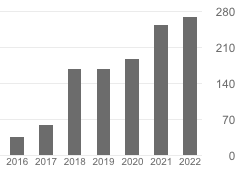
\includegraphics[height=30pt]{scholar-cit.png}

Names of students I supervise(d) are prepended with symbol \student{}.

\subsectionTitle{Pre-prints and In-press}
\begin{pubs}

\wsentry
	{8}
	{Jayanta Mandi, \student{James Kotary}, Senne Berden, Maxime Mulamba, Victor Bucarey, Tias Guns, {\bf Ferdinando Fioretto}} 
	{Decision-Focused Learning: Foundations, State of the Art, Benchmark and Future Opportunities}
	{\venue{Accepted in Journal of Artificial Intelligence Research (JAIR)}, 2024}
	{https://arxiv.org/abs/2307.13565}

\wsentry
	{7}
	{Ethan King, \student{} James Kotary, {\bf Ferdinando Fioretto}, Jan Drgona}
	{Metric Learning to Accelerate Convergence of Operator Splitting Methods for Differentiable Parametric Programming}
	{(under review) \venue{CoRR abs}/2404.00882, 2024}
	{https://arxiv.org/abs/2404.00882}

\wsentry
	{6}
	{\student{} James Kotary, {\bf Ferdinando Fioretto}}
	{Learning Constrained Optimization with Deep Augmented Lagrangian Methods}
	{\venue{CoRR abs}/2403.03454, 2024}
	{https://arxiv.org/abs/2403.03454}

\wsentry
	{5}
	{\student{} Jacob K Christopher, {\bf Ferdinando Fioretto}}
  	{Projected Generative Diffusion Models for Constraint Satisfaction}
	{(under review) \venue{CoRR abs}/2402.03559, 2024}
	{https://arxiv.org/abs/2402.03559}

\wsentry
	{4}
	{\student{} Saswat Das, Marco Romanelli, {\bf Ferdinando Fioretto}}
	{Disparate Impact on Group Accuracy of Linearization for Private Inference}
	{(under review) \venue{CoRR abs}/2402.03629, 2024}
	{https://arxiv.org/abs/2402.03629}

\wsentry
	{3}
	{\student{James Kotary}, \student{Jacob Christopher}, \student{My H Dinh},
	and {\bf Ferdinando Fioretto}}
	{Analyzing and Enhancing the Backward-Pass Convergence of Unrolled Optimization}	
	{(under review) \venue{CoRR abs}/2301.12047, 2024}
	{https://arxiv.org/abs/2301.12047}

\wsentry
	{2}
	{Khang Tran, {\bf Ferdinando Fioretto}, Issa Khalil, My T. Thai, NhatHai Phan} 
	{FairDP: Certified Fairness with Differential Privacy}
	{\venue{CoRR abs}/2305.16474, 2023}
	{https://arxiv.org/abs/2305.16474}

\wsentry
	{1}
	{\student{} Sree Harsha Nelaturu, \student{} Nishaanth Kanna Ravichandran, \student{} Cuong Tran, Sara Hooker, and {\bf Ferdinando Fioretto}}
	{On The Fairness Impacts of Hardware Selection in Machine Learning}	
	{(under review) \venue{CoRR abs}/2312.03886, 2023}
	{https://arxiv.org/abs/2312.03886}
\end{pubs}

\subsectionTitle{Journals}
\begin{pubs}

	\journalentry
	{13}
	{Mostafa Mohammadian, Kyri Baker, \textbf{Ferdinando Fioretto}}
	{Gradient-Enhanced Physics-Informed Neural Networks for Power Systems Operational Support}
	{Electric Power Systems Research (223), pages 109551, 2023}
	{https://www.sciencedirect.com/science/article/abs/pii/S0378779623004406}

	\journalentry
	{12} %{JAIR}
	{Khoi D.~Hoang, \textbf{Ferdinando Fioretto}, Ping Hou, William Yeoh, Makoto Yokoo, Roie Zivan}
	{Proactive Dynamic Distributed Constraint Optimization Problems}
	{\JAIR, (73), pages 179-225, 2022}
	{https://www.jair.org/index.php/jair/article/view/13499}

	\journalentry
	{11} %{AIJ}
		{\textbf{Ferdinando Fioretto}, Pascal Van Hentenryck, Keyu Zhu}
		{Differential Privacy of Hierarchical Census Data: An Optimization Approach}
		{\AIJ, (296), pages 103475, 2021}
		{https://www.sciencedirect.com/science/article/pii/S0004370221000266}

	\journalentryAwd
	{10} %{IEEE-TPS}
		{Vladimir Dvorkin, {\bf Ferdinando Fioretto}, Pascal Van Hentenryck, Pierre Pinson, Jalal Kazempour}
		{Differentially Private Optimal Power Flow for Distribution Grids}
		{\TPS, 36(3), pages 2186--2196, 2021}
		{https://ieeexplore.ieee.org/document/9226144}
		{Best IEEE TPS paper award}
		{(given to 8 out of all TPS papers published in 2019--2021)}

	\journalentry
	{9} %{IEEE-TSG} 
		{{\bf Ferdinando Fioretto}, Terrence W.K.~Mak, Pascal Van Hentenryck}
		{Differential Privacy for Power Grid Obfuscation}
		{\TSG, 11(2), pages 1356--1366, 2020}
		{https://ieeexplore.ieee.org/document/8809257}

	\journalentryAwd
	{8}	%{IEEE-TPS}
		{Terrence W.K.~Mak, {\bf Ferdinando Fioretto}, \student{Lyndon Shi}, Pascal Van Hentenryck}
		{Privacy-Preserving Power System Obfuscation: A Bilevel Optimization Approach}
		{\TPS, 35(2), pages 1627--1637, 2020}
		{https://ieeexplore.ieee.org/document/8854890}
		{Best IEEE TPS paper award}
		{(given to 7 out of all TPS papers published in 2018--2020)}

	\journalentryAwd
	{7}	%{JAIR}
		{{\bf Ferdinando Fioretto}, Pascal Van Hentenryck}
		{OptStream: Releasing Time Series Privately}
		{\JAIR, (65) pages 423--456, 2019}
		{https://www.jair.org/index.php/jair/article/view/11583}
		{Invited to IJCAI 2020 journal track}
		{}

	\journalentryAwd
	{6}	%{IA}
		{{\bf Ferdinando Fioretto}, Agostino Dovier, Enrico Pontelli}
		{Distributed Multi-Agent Optimization for Smart Grids and Home Automation}
		{\venue{Intelligenza Artificiale (IA)},  12 (2), pages: 67--87, 2019}
		{https://content.iospress.com/articles/intelligenza-artificiale/ia180037}
		{Best 2018 Thesis in Artificial Intelligence (AI*IA)}
		{(Accompanying paper)}

	\journalentry
	{5}	%{JAIR}
		{{\bf Ferdinando Fioretto}, Enrico Pontelli, William Yeoh}
		{Distributed Constraint Optimization Problems and Applications: A Survey}
		{\JAIR, 61, pages 623--698, 2018} 
		{https://arxiv.org/abs/1602.06347}

	\journalentry 
	{4}	%{AI Matters}
		{{\bf Ferdinando Fioretto}, William Yeoh}
		{AI Buzzwords Explained: Distributed Constraint Optimization Problems}
		{\venue{AI Matters}, 3 (4), pages 8--13, 2018}
		{https://sigai.acm.org/static/aimatters/3-4/AIMatters-3-4-04-Fioretto.pdf}

	\journalentry 
	{3}	%{Constraints}
		{{\bf Ferdinando Fioretto}, Enrico Pontelli, William Yeoh, Rina Dechter}
		{Accelerating Exact and Approximate Inference for (Distributed) Discrete Optimization with GPUs}
		{\venue{Constraints}, 23 (1), pages 1--43, 2018}
		{https://link.springer.com/article/10.1007/s10601-017-9274-1}

	\journalentry 
	{2}	%{TOMACS}
		{{\bf Ferdinando Fioretto}, Agostino Dovier, Enrico Pontelli}
		{Constrained Community-based Gene Regulatory Network Inference}
		{\venue{ACM Transactions on Modeling and Computer Simulation (TOMACS)}, 25 (2), pages 11:1--11:26, 2015}
		{https://dl.acm.org/doi/10.1145/2688909}

	\journalentry
	{1}	%{JAIR}
		{($\alpha$-$\beta$)\footnote{Author list is order alphabetically.} 
			Federico Campeotto, Alessandro Dal Pal\`{u}, Agostino Dovier,  {\bf Ferdinando Fioretto}, Enrico Pontelli}
		{A Constraint Solver for Flexible Protein Models}
		{\JAIR, 48, pages 953--1000, 2013}
		{https://www.jair.org/index.php/jair/article/view/10856}
\end{pubs}


\subsectionTitle{Rigorously Peer Reviewed Conferences}
\begin{pubs}

%%%%%%%%%%%%%%%%%%%%%%%%%%%%%%%%%%%%%%%%%%%%%%%%%%%%%%%%%%
{\nemph{2024}}&\nemph{\rule{0.5\linewidth}{0.5pt}}\\[1em]

\wsentry
	{63}
	{\student{}My H. Dinh, \student{} James Kotary, {\bf Ferdinando Fioretto}}
	{End-to-End Learning for Fair Multiobjective Optimization Under Uncertainty}
	{\procUAI, 2024}
	{https://arxiv.org/abs/2402.07772}
	{27\%}


\confentry
	{62}%{ArXiv}
	{\student{}Cuong Tran, Keyu Zhu, Pascal Van Hentenryck, {\bf Ferdinando Fioretto}}
	{Fairness Increases Adversarial Vulnerability}
	{\procIJCAI, 2024}
	{https://arxiv.org/abs/2211.11835}
	{13\%?}

\confentry
	{61}
	{\student{} My H.~Dinh, \student{} James Kotary, {\bf Ferdinando Fioretto}}
	{Learning Fair Ranking Policies via Differentiable Optimization of Ordered Weighted Averages}
	{\procFAccT, 2024}
	{https://arxiv.org/abs/2402.05252}
	{unknown}

\confentry
	{60}
	{{\bf Ferdinando Fioretto}, Keyu Zhu, Pascal Van Hentenryck, \student{} Saswat Das and Christine Task}
  	{Finding $\epsilon$ and $\delta$ of Traditional Disclosure Control Systems}
	{\procAAAI, 2024}
	{https://arxiv.org/abs/2301.12204}
	{23.75\%}

%%%%%%%%%%%%%%%%%%%%%%%%%%%%%%%%%%%%%%%%%%%%%%%%%%%%%%%%%%
{\nemph{2023}}&\nemph{\rule{0.5\linewidth}{0.5pt}}\\[1em]

\confentry
	{60}
	{\student{Cuong Tran} and {\bf Ferdinando Fioretto}}
	{Data Minimization at Inference Time}
	{\procNeurIPS, 2023}
	{https://arxiv.org/abs/2305.17593}
	{23\%}

\confentry
	{59}
 	{Vladimir Dvorkin and {\bf Ferdinando Fioretto}}
  	{Price-Aware Deep Learning for Electricity Markets}
  	{Tackling Climate Change with Machine Learning, at NeurIPS 2023}
  	{https://arXiv.org/abs/2308.01436}
  	{35\%}

\confentry
	{58}
	{\student{My H. Dinh}, {\bf Ferdinando Fioretto}, Mostafa Mohammadian, and Kyri Baker}
	{An Analysis of the Reliability of AC Optimal Power Flow Deep Learning Proxies}
	{IEEE PES Innovative Smart Grid Technologies, 2023}
	{https://arxiv.org/abs/2111.11168}
	{unknown}

\confentry 
	{57} %{IJCAI}
	{\student{James Kotary}, \student{My H. Dinh}, {\bf Ferdinando Fioretto}}
	{Folded Optimization for End-to-End Model-Based Learning}
	{\procIJCAI, 2023}
	{https://arxiv.org/abs/2301.12047}
	{15\%}

\confentry
    {56} %{IJCAI}
	{\student{James Kotary}, \student{Vincenzo Di Vito}, {\bf Ferdinando Fioretto}, Pascal Van Hentenryck}
	{SF-PATE: Scalable, Fair, and Private Aggregation of Teacher Ensembles}
    {\procIJCAI, 2023}
	{https://arxiv.org/abs/2204.05157}
    {15\%}

\confentry
    {55} %{IJCAI}
	{\student{James Kotary}, \student{Vincenzo Di Vito}, {\bf Ferdinando Fioretto}}
	{End-to-End Combinatorial Ensemble Learning}
    {\procIJCAI, 2023}
	{http://arxiv.org/abs/2211.00251}
    {15\%}

\confentry
    {54} %{IJCAI}
	{\student{Cuong Tran}, {\bf Ferdinando Fioretto}}
	{On the Fairness Impacts of Private Ensembles Models}
    {\procIJCAI, 2023}
	{http://arxiv.org/abs/2109.08630}
    {15\%}

\confentry
	{53} %{PES}
	{Terrence W.K. Mak, {\bf Ferdinando Fioretto}, Pascal Van Hentenryck}
	{Load Encoding for Learning AC-OPF}
	{Proceedings of the \venue{IEEE PES General Meeting (PES)}, 2023}
	{https://arxiv.org/abs/2101.03973}
	{N/A}

\confentry
    {52} %{AAMAS}
	{\student{James Kotary}, \student{Vincenzo Di Vito}, {\bf Ferdinando Fioretto}}
	{End-to-End Optimization and Learning for Multiagent Ensembles}
    {\procAAMAS, 2023}
	{http://arxiv.org/abs/2211.00251}
    {40\%}

%%%%%%%%%%%%%%%%%%%%%%%%%%%%%%%%%%%%%%%%%%%%%%%%%%%%%%%%%%
{\nemph{2022}}&\nemph{\rule{0.5\linewidth}{0.5pt}}\\[1em]

\confentryAwd
	{51} %{NeurIPS}
	{\student{Cuong Tran}, {\bf Ferdinando Fioretto}, Jung-Eun Kim, \student{Rakshit Naidu}}
	{Pruning has a disparate impact on model accuracy}
	{\procNeurIPS, 2022}
	{http://arxiv.org/abs/2205.13574}
	{25.6\%}
	{Lightning Talk (Spotlight)}
	{(Typically assigned to $\sim$3\% out of all paper submissions (10,411, in 2022))}

	\confentry
	{50} %{IJCAI}
	{Keyu Zhu, {\bf Ferdinando Fioretto}, Pascal Van Hentenryck}
	{Post-processing of Differentially Private Data: A Fairness Perspective}
	{\procIJCAI, 2022}
	{http://arxiv.org/abs/2202.09425}	
	{15\%}

	\confentry
	{49} %{IJCAI}
	{{\bf Ferdinando Fioretto}, \student{Cuong Tran}, Keyu Zhu, Pascal Van Hentenryck}
	{Differential Privacy and Fairness in Decisions and Learning Tasks: A Survey}
	{\procIJCAI, 2022}
	{http://arxiv.org/abs/2202.08187}	
	{18\% (survey track)}

	\confentryAwd
	{48} %{IJCAI}
	{{\bf Ferdinando Fioretto}}
	{Integrating Machine Learning and Optimization to Boost Decision Making}
	{\procIJCAI, 2022}
	{https://web.ecs.syr.edu/~ffiorett/files/papers/Fioretto-IJCAI22-EC.pdf}	
	{Invited}
	{Early Career Spotlight}
	{(Accompanying paper)}

	\confentry
	{47} %{WWW}
	{\student{James Kotary}, {\bf Ferdinando Fioretto}, Pascal Van Hentenryck, Ziwei Zhu}
	{End-to-end Learning for Fair Ranking Systems}
	{\procWWW, 2022}
	{http://arxiv.org/abs/2111.10723}	
	{17\%}
	
	\confentry
	{46} %{AAAI} 
	{\student{James Kotary}, {\bf Ferdinando Fioretto}, Pascal Van Hentenryck}
	{Fast Approximations for Job Shop Scheduling: A Lagrangian Dual Deep Learning Method}
	{\procAAAI, 2022}
	{http://arxiv.org/abs/2110.06365}
	{15\%}

	\confentry
	{45} %{PMAPS}
	{Lesia Mitridati, Emma Romei, Gabriela Hug, {\bf Ferdinando Fioretto}}
	{Differentially-Private Heat and Electricity Markets Coordination}
	{\procPMAPS, 2022}
	{https://arxiv.org/abs/2201.10634}
	{N/A}
 
	\confentry
	{44} %{PMAPS}
	{Mostafa Mohammadian, Kyri Baker, \student{My H.~Dinh}, {\bf Ferdinando Fioretto}}
	{Learning Solutions for Intertemporal Power Systems Optimization with Recurrent Neural Networks}
	{\procPMAPS, 2022}
	{N/A}


%%%%%%%%%%%%%%%%%%%%%%%%%%%%%%%%%%%%%%%%%%%%%%%%%%%%%%%%%%
{\nemph{2021}}&\nemph{\rule{0.5\linewidth}{0.5pt}}\\[1em]

	\confentry 
	{43} %{NeurIPS}
	{\student{Cuong Tran}, \student{My H. Dinh}, {\bf Ferdinando Fioretto}}
	{Differentially Private Deep Learning under the Fairness Lens}
	{\procNeurIPS, 2021}
	{https://arxiv.org/pdf/2106.02674.pdf}
	{26\%} % 9122

	\confentry 
	{42} %{NeurIPS}
	{\student{James Kotary}, {\bf Ferdinando Fioretto}, Pascal Van Hentenryck}
	{Learning Hard Optimization Problems: A Data Generation Perspective}
	{\procNeurIPS, 2021}
	{https://arxiv.org/pdf/2106.02674.pdf}
	{26\%} % 9122

	\confentryAwd 
	{41} %{IJCAI}
	{\student{Cuong Tran}, {\bf Ferdinando Fioretto}, Pascal Van Hentenryck, \student{Zhiyan Yao}}
	{Decision Making with Differential Privacy under the Fairness Lens}
	{\procIJCAI, 560--566, 2021}
	{https://www.ijcai.org/proceedings/2021/78}
	{13.9\%} %4,204/587
	{2022 Caspar Bowden PET Award}
	{(Selected among all papers about Privacy Enhancing Technologies published in international conferences between 2020--2022.)}

	\confentry 
	{40} %{IJCAI}
	{\student{James Kotary}, {\bf Ferdinando Fioretto}, Pascal Van Hentenryck, Bryan Wilder}
	{End-to-End Constrained Optimization Learning: A Survey}
	{\procIJCAI, 4475--4482, 2021}
	{https://www.ijcai.org/proceedings/2021/610}
	{30.1\%}

	\confentry 
	{39} %{AAAI}
	{Keyu Zhu, Pascal Van Hentenryck, {\bf Ferdinando Fioretto}}
	{Bias and Variance of Post-processing in Differential Privacy}
	{\procAAAI, 11177--11184, 2021}
	{https://ojs.aaai.org/index.php/AAAI/article/view/17333}
    {21.0\%} %  7,911/1,692

	\confentry 
	{38} %{AAAI}
	{\student{Cuong Tran}, {\bf Ferdinando Fioretto}, Pascal Van Hentenryck}
	{Differentially Private and Fair Deep Learning: A Lagrangian Dual Approach}
	{\procAAAI, 9932--9939, 2021}
	{https://ojs.aaai.org/index.php/AAAI/article/view/17193}
    {21.0\%} %  7,911/1,692

    \confentry
    {37} %{AAMAS}
    {\student{Anudit Nagar}, \student{Cuong Tran}, {\bf Ferdinando Fioretto}}
    {A Privacy-Preserving and Accountable Multi-agent Learning Framework}
    {\procAAMAS, 1605--1606, 2021}
    {https://dl.acm.org/doi/10.5555/3463952.3464174}
    {40\%}

	\confentry
	{36} %{CP}
	{\bf Ferdinando Fioretto}
	{Constrained-based Differential Privacy}
	{\procCP, 1868--8969, 2021}
	{https://drops.dagstuhl.de/opus/volltexte/2021/15293/}
	{Invited}
	
	\confentry 
	{35} %{PowerTech}
	{Vladimir~Dvorkin, {\bf Ferdinando Fioretto}, Pascal Van Hentenryck, Jalal~Kazempour, Pierre~Pinson}
	{Differentially Private Optimal Power Flow for Distribution Grids}
	{\venue{IEEE PowerTech}, 2021}
	{https://ieeexplore.ieee.org/document/9226144}
	{N/A} %4,204/587

%%%%%%%%%%%%%%%%%%%%%%%%%%%%%%%%%%%%%%%%%%%%%%%%%%%%%%%%%%
{\nemph{2020}}&\nemph{\rule{0.5\linewidth}{0.5pt}}\\[1em]
	\confentry
		{34} %{ECML}
		{{\bf Ferdinando Fioretto}, Pascal Van Hentenryck, Terrence W.K. Mak, \student{Cuong Tran}, Federico Baldo, Michele Lombardi} 
		{A Lagrangian Dual Framework for Deep Neural Networks with Constraints}
		{\procECML, 18--135, 2020}
		{https://arxiv.org/abs/2001.09394}
		{19\%}

	\confentry
		{33} %{IJCAI}
		{{\bf Ferdinando Fioretto}, Lesia Mitridati, Pascal Van Hentenryck}
		{Differential Privacy Stackebelg Games}
		{\procIJCAI, 3480--3486, 2020}
		{https://www.ijcai.org/proceedings/2020/0481.pdf}
	    {12.6\%}

	\confentryAwd
		{32} %{IJCAI}
		{{\bf Ferdinando Fioretto}, Pascal Van Hentenryck}
		{OptStream: Releasing Time Series Privately}
		{\procIJCAI, 5135--5139, 2020}
	    {https://www.ijcai.org/proceedings/2020/722}
		{invited}
		{Invited to the IJCAI journal track}{}
	
	\confentry
		{31} %{PSCC}
		{Terrence W.K.~Mak, {\bf Ferdinando Fioretto}, Pascal Van Hentenryck}
		{Privacy-Preserving Obfuscation for Distributed Power Systems}
		{\procPSCC, 2020}
		{https://arxiv.org/abs/1910.04250}
	    {$\sim$30\%} %  7,737/1591

	\confentry
		{30} %{AAAI}
		{{\bf Ferdinando Fioretto}, Terrence W.K.~Mak, Pascal Van Hentenryck}
		{Predicting AC Optimal Power Flows: Combining Deep Learning and Lagrangian Dual Methods}
	  	{\procAAAI, pages 630--637, 2020}
	  	{https://ojs.aaai.org//index.php/AAAI/article/view/5403}
	    {20.6\%} %  7,737/1591

	\confentry
		{29} %{PRIMA}
	    {Atena Tabakhi, William Yeoh, {\bf Ferdinando Fioretto}}
	    {The Smart Appliance Scheduling Problem: A Bayesian Optimization Approach}
	    {\procPRIMA, 100--115, 2020}
	    {https://link.springer.com/chapter/10.1007\%2F978-3-030-69322-0\_7}
	    {38.0\%} % 19/50

%%%%%%%%%%%%%%%%%%%%%%%%%%%%%%%%%%%%%%%%%%%%%%%%%%%%%%%%%%
{\nemph{2019}}&\nemph{\rule{0.5\linewidth}{0.5pt}}\\[1em]
	\confentry
		{28} %{AAMAS}
		{{\bf Ferdinando Fioretto}, Pascal Van~Hentenryck}
		{Privacy-Preserving Federated Data Sharing}
	  	{\procAAMAS, pages 638--646, 2019}
	  	{https://dl.acm.org/doi/abs/10.5555/3306127.3331750}
		{24\%} % 189/781

	\confentry
		{27} %{IJCAI}
		{{\bf Ferdinando Fioretto}, Terrence W.K.~Mak, Pascal Van Hentenryck}
		{Privacy-Preserving Obfuscation of Critical Infrastructure Networks}
	  	{\procIJCAI, pages 1086--1092, 2019}
	  	{https://www.ijcai.org/proceedings/2019/0152.pdf}
	    {17.9\%} %  4,752/850

	\confentryAwd
		{26} %{CP}
		{{\bf Ferdinando Fioretto}, Pascal Van Hentenryck}
		%\href{https://web.ecs.syr.edu/~ffiorett/files/papers/cp19.pdf}
		{Differential Privacy of Hierarchical Census Data: An Optimization Approach} 
		{\procCP, pages 639--655, 2019}
		{https://link.springer.com/chapter/10.1007/978-3-030-30048-7\_37}
		{37\%}
		{Invited to Constraint journal}
		{(selected papers -- declined)}

%%%%%%%%%%%%%%%%%%%%%%%%%%%%%%%%%%%%%%%%%%%%%%%%%%%%%%%%%%
{\nemph{2018}}&\nemph{\rule{0.5\linewidth}{0.5pt}}\\[1em]
	\confentry 
		{25} %{PRIMA}
		{{\bf Ferdinando Fioretto}, Hong Xu, Sven Koenig, TK Satish Kumar}
	 	{Solving Multiagent Constraint Optimization Problems on the Constraint Composite Graph}
		{\procPRIMA, pages 106--122, 2018}
		{https://link.springer.com/chapter/10.1007/978-3-030-03098-8\_7}
	    {26\%} % 27/103

	\confentry
		{24} %{AAMAS}
	  	{{\bf Ferdinando Fioretto}, Chansoo Lee, Pascal Van Hentenryck}
	  	{Constrained-based Differential Privacy for Private Mobility} 
	  	{\procAAMAS, pages 1405--1413, 2018}
	  	{https://dl.acm.org/doi/abs/10.5555/3237383.3237910}
	    {25\%} % 151/597

	\confentry 
		{23} %{CP}
		{Khoi Hoang, {\bf Ferdinando Fioretto}, William Yeoh, Enrico Pontelli, Roie Zivan}
		{A Large Neighboring Search Schema for Multi-Agent Optimization}
		{\procCP, pages 688--706, 2018}
		{https://link.springer.com/chapter/10.1007/978-3-319-98334-9\_44}
	    {33\%} % 3/9 (in this track)

	\confentry 
		{22} %{CPAIOR}
		{{\bf Ferdinando Fioretto}, Pascal Van Hentenryck}
		{Constrained-based Differential Privacy: Releasing Optimal Power Flow Benchmarks Privately} 
		{\procCPAIOR, pages 215--231, 2018}
		{https://link.springer.com/chapter/10.1007/978-3-319-93031-2\_15}
	    {48\%}

	\confentry
		{21} %{ISIAM}
		{{\bf Ferdinando Fioretto}, Hong Xu, Sven Koenig, TK Satish Kumar}
		{Constraint Composite Graph-Based Lifted Message Passing for Distributed Constraint Optimization Problems}
		{\procISIAM, 2018}
		{https://speakerdeck.com/xuphys/constraint-composite-graph-based-lifted-message-passing-for-distributed-constraint-optimization-problems}
		{N/A}

%%%%%%%%%%%%%%%%%%%%%%%%%%%%%%%%%%%%%%%%%%%%%%%%%%%%%%%%%%
{\nemph{2017}}&\nemph{\rule{0.5\linewidth}{0.5pt}}\\[1em]
	\confentry 
		{20} %{AAMAS}
		{{\bf Ferdinando Fioretto}, William Yeoh, Enrico Pontelli, Ye Ma, Satishkumar J.~Ranade}
		{A Distributed Constraint Optimization (DCOP) Approach to the Economic Dispatch with Demand Response}
		{\procAAMAS, pages  999--1007, 2017}
		{https://dl.acm.org/doi/10.5555/3091125.3091267}
		{25\%}%{\it 137/550 = 25\%}.

	\confentry 
		{19} %{AAMAS}
		{{\bf Ferdinando Fioretto},  William Yeoh, Enrico Pontelli}
		{A Multiagent System Approach to Scheduling Devices in Smart Homes}
		{\procAAMAS, pages 981--989, 2017} 
		{https://dl.acm.org/doi/10.5555/3091125.3091265}
		{25\%}%{\it 137/550 = 25\%}

	\confentry
		{18} %{AAMAS} 
		{Khoi Hoang, Ping Hou, {\bf Ferdinando Fioretto}, Makoto Yokoo, William Yeoh, Roie Zivan}
		{Infinite-Horizon Proactive Dynamic DCOPs}
		{\procAAMAS, pages 212--220, 2017}
		{https://dl.acm.org/doi/10.5555/3091125.3091160}
		{25\%}%{\it 137/550 = 25\%}.

	\confentry 
		{17} %{CP}
		{Atena M.~Tabakhi, Tiep Le, {\bf Ferdinando Fioretto}, William Yeoh}
		{Preference Elicitation for DCOPs}
		{\procCP, pages 278--296, 2017}
		{https://link.springer.com/chapter/10.1007/978-3-319-66158-2\_18}
		{43\%}%{\it 50+4/(137+17) = 25\%}.

%%%%%%%%%%%%%%%%%%%%%%%%%%%%%%%%%%%%%%%%%%%%%%%%%%%%%%%%%%
{\nemph{2016}}& \nemph{\rule{0.5\linewidth}{0.5pt}}\\[1em]
	\confentry 
		{16} %{AAMAS}
		{Khoi Hoang, {\bf Ferdinando Fioretto}, Ping Hou, Makoto Yokoo, William Yeoh, Roie Zivan}
		{Proactive Dynamic Distributed Constraint Optimization Problems} 
		{\procAAMAS, pages 597--605, 2016}
		{https://www.ifaamas.org/Proceedings/aamas2019/pdfs/p2411.pdf}
		{25\%}%{\it 137/550 = 25\%}.

	\confentry 
		{15} %{AAMAS}
		{Tiep Le, {\bf Ferdinando Fioretto}, William Yeoh, Enrico Pontelli, Tran Cao Son} 
		{ER-DCOPs: A Framework for Distributed Constraint Optimization Problems With Uncertainty} 
		{\procAAMAS,	pages 606--614, 2016}
		{https://dl.acm.org/doi/10.5555/2936924.2937014}
		{25\%}%{\it 137/550 = 25\%}.

	\confentry 
		{14} %{AAAI}
		{{\bf Ferdinando Fioretto}, William Yeoh, Enrico Pontelli}
		{Multi-Variable Agent Decompositions for DCOPs}
		{\procAAAI, pages 2480--2486, 2016}
		{https://dl.acm.org/doi/10.5555/3016100.3016246}
		{26\%}%{\it 549/2132 = 26\%}.

	\confentry
		{13} %{CP} 
		{{\bf Ferdinando Fioretto}, William Yeoh, Enrico Pontelli}
		{A Dynamic Programming-Based MCMC Framework for Solving DCOPs with GPUs}
		{\procCP, pages 813--831,	2016}
		{https://link.springer.com/chapter/10.1007/978-3-319-44953-1\_51}
		{35\%}%{\it 50+4/(137+17) = 34\%}.

%%%%%%%%%%%%%%%%%%%%%%%%%%%%%%%%%%%%%%%%%%%%%%%%%%%%%%%%%%
{\nemph{2015}}&\nemph{\rule{0.5\linewidth}{0.5pt}}\\[1em]
	\confentry
		{12} %{CP}
		{{\bf Ferdinando Fioretto}, Tiep Le, Enrico Pontelli, William Yeoh, Tran Cao Son}
		{Exploiting GPUs in Solving (Distributed) Constraint Optimization Problems with Dynamic Programming}
		{\procCP, pages 121--139, 2015}
		{https://dl.acm.org/doi/10.5555/3102787.3102797}
		{49\%}%{\it  39/80 = 49\%}.

	\confentry
		{11} %{AAMAS}
		{{\bf Ferdinando Fioretto}, Federico Campeotto, Agostino Dovier, Enrico Pontelli, William Yeoh}
		{Large Neighborhood Search with Quality Guarantees for Distributed Constraint Optimization Problems}
		{\procAAMAS, pages 1835--1836, 2015}
		{https://dl.acm.org/doi/10.5555/2772879.2773461}
		{46\%}

	\confentry
		{10} %{AAMAS}
		{{\bf Ferdinando Fioretto}, William Yeoh, Enrico Pontelli}
		{Multi-Variable Agents Decomposition for DCOPs to Exploit Multi-Level Parallelism}
		{\procAAMAS, pages 1823--1824, 2015}
		{https://dl.acm.org/doi/10.5555/2772879.2773455}
		{46\%}

	\confentry
		{9} %{AAMAS}
		{{\bf Ferdinando Fioretto}}
		{Exploiting the Structure of Distributed Constraint Optimization Problems} 
		{\procAAMAS, pages 2007--2008, 2015}
		{https://dl.acm.org/doi/10.5555/2772879.2773549}
		{N/A}

	\confentry
		{8} %{AAAI}
		{{\bf Ferdinando Fioretto}} 
		{Exploiting the Structure of Distributed Constraint Optimization Problems}
		{\procAAAI,  pages 4233--4234, 2015}
		{https://www.aaai.org/ocs/index.php/AAAI/AAAI15/paper/view/9293}
		{N/A}

%%%%%%%%%%%%%%%%%%%%%%%%%%%%%%%%%%%%%%%%%%%%%%%%%%%%%%%%%%
{\nemph{$\leq$2014}}&\nemph{\rule{0.5\linewidth}{0.5pt}}\\[1em]
	\confentry 
		{7} %{ECAI}
		{($\alpha$-$\beta$) 
		Federico Campeotto, Agostino Dovier, {\bf Ferdinando Fioretto}, Enrico Pontelli}
		{A GPU Implementation of Large Neighborhood Search for Solving Constraint Optimization Problems} 
		{\procECAI, pages 189--194, 2014}
		{https://dl.acm.org/doi/10.5555/3006652.3006685}
		{28\%}

	\confentry
		{6} %{CP}
		{{\bf Ferdinando Fioretto}, Tiep Le, William Yeoh, Enrico Pontelli, Tran Cao Son}
		{Improving DPOP with Branch Consistency for Solving Distributed Constraint Optimization Problems}
		{\procCP, pages 307--323, 2014}
		{https://link.springer.com/chapter/10.1007\%2F978-3-319-10428-7\_24}
		{50\%}
		
	\confentry
		{5} %{PADL}
		{($\alpha$-$\beta$) 
		Federico Campeotto, Alessandro Dal Pal\`{u}, Agostino Dovier, {\bf Ferdinando Fioretto}, Enrico Pontelli}
		{Exploring the Use of GPUs in Constraint Solving}
		{\procPADL, pages 152--167, 2014}
		{https://link.springer.com/chapter/10.1007\%2F978-3-319-04132-2\_11}
		{55\%}

	\confentry 
		{4} %{AAMAS}
		{{\bf Ferdinando Fioretto}, Federico Campeotto, Luca Da Rin Fioretto, William Yeoh, Enrico Pontelli} 
		{GD-Gibbs: A GPU-based Sampling Algorithm for Solving Distributed Constraint Optimization Problems} %(Extended Abstract)". 
		{\procAAMAS, pages 1339--1340, 2014}
		{https://dl.acm.org/doi/10.5555/2615731.2617462}
		{46\%}
	
	\confentryAwd
		{3} %{CMSB}
		{{\bf Ferdinando Fioretto}, Enrico Pontelli} 
		{Constraint Programming in Community-based Gene Regulatory Network Inference} 
		{\procCMSB, pages 135--149, 2013}
		{https://link.springer.com/chapter/10.1007\%2F978-3-642-40708-6\_11}
		{55\%}
		{Best Student Paper Award}{}

	\confentry 
		{2} %{CP}
		{($\alpha$-$\beta$) 
		Federico Campeotto, Alessandro Dal Pal\`{u}, Agostino Dovier, {\bf Ferdinando Fioretto}, Enrico Pontelli}
		{A Filtering Technique for Fragment Assembly-based Proteins Loop Modeling with Constraints} 
		{\procCP, pages 850--866, 2012}
		{https://link.springer.com/chapter/10.1007\%2F978-3-642-33558-7\_61}
		{36\%}

	\confentry
		{1} % {Neuroscience}
		{Michael R. Best, {\bf Ferdinando Fioretto}, Alessandro Dal Pal\`{u}, Enrico Pontelli, Tran Son, TuShun R. Powers, Elba E. Serrano}
		{The role of secondary and tertiary structure prediction in determining the function of novel genes found in Xenopus Leavis}
		{\venue{Neuroscience}, 2011, (518.20/ZZ45)}{}
		{N/A}
\end{pubs}

\subsectionTitle{Book Chapters and Editorial Articles}
\begin{pubs}
\journalentry
	{5} %{AI Mag.}
	{{\bf Ferdinando Fioretto}, et al.} 
	{Reports of the Workshops Held at the 2022 AAAI Conference on Artificial Intelligence}
	{{\bf AI Magazine}, 2022}
	{https://interactiveaimag.org/updates/reports/reports-of-the-workshops-held-at-the-2022-aaai-conference-on-artificial-intelligence/}

\journalentry
	{4} %{AI Mag.}
	{{\bf Ferdinando Fioretto}, et al.} 
	{Reports of the Workshops Held at the 2021 AAAI Conference on Artificial Intelligence}
	{{\bf AI Magazine}, 2021}
	{https://interactiveaimag.org/updates/reports/reports-of-the-workshops-held-at-the-2021-aaai-conference-on-artificial-intelligence/}

\journalentry
	{3} %{AI Mag.}
	{{\bf Ferdinando Fioretto}, et al.} 
	{Reports of the Workshops Held at the 2020 International Association for the Advancement of Artificial Intelligence Conference on Web and Social Media}
	{{\bf AI Magazine},  41(4) 2020}
	{https://ojs.aaai.org/index.php/aimagazine/article/view/7486}

\journalentryAwd
	{2} %{LNCS}
	{\student{William Kluegel}, \student{Muhammad A.~Iqbal}, {\bf Ferdinando Fioretto}, William Yeoh, Enrico Pontelli}
	{A Realistic Dataset for the Smart Home Device Scheduling Problem for DCOPs}
	{\emph{Lecture Notes in Computer Science (LCNS)}, LNCS, volume 10643 pages 125--142, Springer, 2017}
	{https://link.springer.com/chapter/10.1007\%2F978-3-319-71679-4\_9}
	{Visionary Paper Award}
	{(AAMAS workshop series)}

\journalentry
	{1} %{LNBIP}
	{Moinul M.P.~Chowdhury, Russell Y.~Folk, {\bf Ferdinando Fioretto}, Christopher Kiekintveld, William Yeoh}
	{Investigation of Learning Strategies for the SPOT Broker in Power TAC}
	{\emph{AgentMediated Electronic Commerce: Designing Trading Strategies and Mechanisms for Electronic Markets}, volume 271 of Lecture Notes in Business Information Processing, 
	    pages 96–111, Springer, 2017}
    {https://link.springer.com/chapter/10.1007\%2F978-3-319-54229-4\_7}
\end{pubs}


\subsectionTitle{Workshops \& Presentations}
\begin{pubs}
\wsentry 
	{21}%{ArXiv}
	{Vladimir Dvorkin, {\bf Ferdinando Fioretto}, Pascal Van Hentenryck, Pierre Pinson, Jalal Kazempour}
	{Privacy-Preserving Convex Optimization: When Differential Privacy Meets Stochastic Programming}
	{\venue{Workshop on Climate Change AI -- at NeurIPS}, 2023}
	{http://arxiv.org/abs/2209.14152}


	\wsentryAwd
	{20} %{PPAI}
	{\student{Cuong Tran}, \student{My H.~Dinh}, {\bf Ferdinando Fioretto}}
	{A Fairness Analysis on Private Aggregation of Teacher Ensembles}
	{\venue{AAAI Workshop on Privacy Preserving Artificial Intelligence 
		(PPAI)--at AAAI}, 2022}
	{http://arxiv.org/abs/2109.08630}
	{Spotlight Paper}
	
	\wsentry
	{19} %{TPDP}
	{\student{Cuong Tran}, {\bf Ferdinando Fioretto}}
	{Decision Making with Differential Privacy under the Fairness Lens}
	{\venue{Theory and Practice of Differential Privacy (TPDP) -- at ICML}, 2021}
	{https://tpdp.journalprivacyconfidentiality.org/2021/}
 	
	\wsentry
	{18} %{OptLMAS}
	{\student{Anudit Nagar}, \student{Cuong Tran}, {\bf Ferdinando Fioretto}}
	{A Privacy-Preserving and Accountable Multi-agent Learning Framework}
	{\venue{International Workshop on Learning and Optimization 
 		   in Multi-Agent Systems (OPTLearnMAS)--at AAMAS}, 2021}
	{https://optlearnmas21.github.io/}

	\wsentry
	{17} %{PPAI}
	{\student{Cuong Tran}, {\bf Ferdinando Fioretto}, Pascal Van 	Hentenryck}
	{Differentially Private and Fair Deep Learning: A Lagrangian Dual Approach}
	{\venue{AAAI Workshop on Privacy Preserving Artificial Intelligence 
		(PPAI)--at AAAI}, 2021}
	{https://arxiv.org/abs/2009.12562}

\wsentry 
	{16} %{INFORMS}
	{{\bf Ferdinando Fioretto}, \student{Cuong Tran}, Pascal Van Hentenryck}
	{Lagrangian Duality for Constrained Deep Learning}
	{\venue{INFORMS}, 2020}
	{http://meetings2.informs.org/wordpress/annual2020/}

\wsentry 
	{15} %{INFORMS}
	{Lesia Mitridati, {\bf Ferdinando Fioretto}, Pascal Van Hentenryck}
	{Differential Privacy For Stackelberg Games: An Application To Gas And Electricity Markets}
	{\venue{INFORMS}, 2020}
	{http://meetings2.informs.org/wordpress/annual2020/}


\wsentry 
	{14} %{OptMAS}
	{Khoi Hoang, {\bf Ferdinando Fioretto}, William Yeoh, Enrico Pontelli, Roie Zivan}
	{A Large Neighboring Search Schema for Multi-Agent Optimization} 
	{\venue{International Workshop on Optimization 
 		   in Multi-Agent Systems (OPTMAS)--at AAMAS}, 2019}
	{https://www2.isye.gatech.edu/~fferdinando3/cfp/OPTMAS19/}

\wsentry
	{13} %{OptMAS}
	{{\bf Ferdinando Fioretto}, Hong Xu, Sven Koenig, TK Satish Kumar}
	{Solving Multiagent Constraint Optimization Problems on the Constraint Composite Graph} 
	{\venue{International Workshop on Optimisation in Multi-Agent Systems 
	(OptMAS)--at AAMAS}, 2018}
	{~}

\wsentry
	{12} %{OptMAS}	
	{William Kluegel, Muhammad Aamir Iqbal, {\bf Ferdinando Fioretto}, William Yeoh, Enrico Pontelli}
	{A Realistic Dataset for the Smart Home Device Scheduling Problem for DCOPs}
	{\venue{International Workshop on Optimisation in Multi-Agent Systems (OPTMAS)--at AAMAS}, 
	2017}
	{~}	

\wsentry
	{11} %{AISGSB}
	{{\bf Ferdinando Fioretto},  William Yeoh, Enrico Pontelli}
	{A Multiagent System Approach to Scheduling Devices in Smart Homes}
	{\venue{Workshop on AI for Smart Grids and Smart Buildings (AISGSB)--at AAAI}, 2017}
	{~}

	\wsentry
	{10} %{MPREF} 
	{Atena M.~Tabakhi, {\bf Ferdinando Fioretto}, William Yeoh}
	{A Preliminary Study on Preference Elicitation in DCOPs for Scheduling Devices in Smart Buildings}
	{\venue{10th Workshop on Advances in Preference Handling (MPREF)--at IJCAI}, 2016}
	{~}

\wsentry 
	{9} %{TADA}
	{Porag Chowdhury, Russell Y. Folk, {\bf Ferdinando Fioretto}, Christopher Kiekintveld, William Yeoh}
	{Investigation of Learning Strategies for the SPOT Broker in Power TAC}
  	{\venue{International Workshop on Agent Mediated Electronic Commerce and Trading Agents Design and Analysis
	(AMEC/TADA)--at AAMAS}, 2016}
	{~}

\wsentry 
	{8} %{AISGSB}
	{Khoi Hoang, {\bf Ferdinando Fioretto}, Ping Hou, Makoto Yokoo, William Yeoh, Roie Zivan}
	{Proactive Dynamic DCOPs} 
	{\venue{Workshop on AI for Smart Grids and Smart Buildings (AISGSB)--at AAAI}, 2016}
	{~}	

\wsentry
	{7} %{OptMAS} 
	{{\bf Ferdinando Fioretto}, Federico Campeotto, Agostino Dovier, Enrico Pontelli, William Yeoh}
	{Large Neighborhood Search with Quality Guarantees for Distributed Constraint Optimization Problems} 
	{In \venue{International Workshop on Optimization in Multi-Agent Systems (OptMAS)-- at AAMAS}, 2015}
	{~}

\wsentry 
	{6} %{OptMAS}
	{{\bf Ferdinando Fioretto}, Tiep Le, William Yeoh, Enrico Pontelli, Tran Cao Son}
	{Improving DPOP with Branch Consistency for Solving Distributed Constraint Optimization Problems}
	{In \venue{International Workshop on Optimization in Multi-Agent Systems (OptMAS)-- at AAMAS}, 2015}
	{~}

\wsentry 
	{5} %{WCB}
	{($\alpha$-$\beta$) 
	Federico Campeotto, Alessandro Dal Pal\`{u}, Agostino Dovier, {\bf Ferdinando Fioretto}, Enrico Pontelli} 
  	{Experimenting with FIASCO for protein structure prediction}
	{\venue{Workshop on Constraint Based Methods for Bioinformatics (WCB)--at CP}, 2014}
	{~}

\wsentry 
	{4} %{ParSeachOpt}
	{($\alpha$-$\beta$) Federico Campeotto, Alessandro Dal Pal\`{u}, Agostino Dovier, {\bf Ferdinando Fioretto}, Enrico Pontelli}
	{Towards a complete constraint solver on GPU}
	{In \venue{Workshop on Parallel Methods for Search \& Optimization (ParSearchOpt)--at ECAI}, 2014}
	{~}

\wsentry 
	{3} %{WCB}
	{{\bf Ferdinando Fioretto}, Enrico Pontelli}
	{Community-based Gene Regulatory Network Inference via Constraint Programming}
	{\venue{Workshop on Constraint Based Methods for Bioinformatics (WCB)--at CP}, 2013}
	{~} 

\wsentry
	{2} %{WCB} 
	{($\alpha$-$\beta$) 
	Federico Campeotto, Alessandro Dal Pal\`{u}, Agostino Dovier, {\bf Ferdinando Fioretto}, Enrico Pontelli}
	{Protein Loop Modelling via Constraints and Fragment Assembly}
	{\venue{Workshop on Constraint Based Methods for Bioinformatics (WCB)--at CP}, 2012}
	{~} 

\wsentry 
	{1} %{WCB}
	{($\alpha$-$\beta$) 
	Michael R. Best, Kabi Bhattarai, Federico Campeotto, Alessandro Dal Pal\`{u}, Hung Dang, Agostino Dovier, {\bf Ferdinando Fioretto}, Federico Fogolari, Tiep Le, Enrico Pontelli}
		{Introducing FIASCO: Fragment-based Interactive Assembly for protein Structure prediction with COnstraints}
 	 {\venue{Workshop on Constraint Based Methods for  Bioinformatics (WCB)--at CP}, 2011}
  	{~}
\end{pubs}

%--------------------------------------------------------------------
%	Conference: Archieved Papers
%--------------------------------------------------------------------
\subsectionTitle{Archived and Extended Versions of Published Papers}
\begin{pubs}

\wsentry 
	{12}%{ArXiv}
	{\student{My H. Dinh}, {\bf Ferdinando Fioretto}}
	{Context-Aware Differential Privacy for Language Modeling}
	{\venue{CoRR abs}/2301.12288, 2023}
	{https://arxiv.org/abs/2301.12288}

\wsentry 
	{11}%{ArXiv}
	{Sawinder Kaur, {\bf Ferdinando Fioretto}, Asif Salekin}
	{Deadwooding: Robust Global Pruning for Deep Neural Networks} 
	{\venue{CoRR abs}/2202.05226, 2022}
	{http://arxiv.org/abs/2202.05226}

\wsentry 
	{10}%{ArXiv}
	{\student{My H.~Dinh}, {\bf Ferdinando Fioretto}, Mostafa Mohammadian, Kyri Baker}
	{Towards Understanding the Unreasonable Effectiveness of Learning AC-OPF Solutions}
	{\venue{CoRR abs}/2111.11168, 2021}
	{http://arxiv.org/abs/2111.11168}

% \wsentry 
% 	{10}%{ArXiv}
% 	{\student{Cuong Tran}, \student{My H.~Dinh}, \student{Kyle Beiter}, {\bf Ferdinando Fioretto}}
% 	{A Fairness Analysis on Private Aggregation of Teacher Ensembles}
% 	{\venue{CoRR abs}/2109.08630, 2021}
% 	{http://arxiv.org/abs/2109.08630}

\wsentry % (NeruIPS-21)
	{9}%{ArXiv}
	{\student{Cuong Tran}, \student{My H.~Dinh}, {\bf Ferdinando Fioretto}}
	{Differentially Private Deep Learning under the Fairness Lens}
	{\venue{CoRR abs}/2106.02674, 2021 ({\bf extended NeurIPS-21 version})}
	{http://arxiv.org/abs/2106.02674}

\wsentry 
	{8}%{ArXiv}
	{\student{Anudit Nagar}, \student{Cuong Tran}, {\bf Ferdinando Fioretto}}
	{A Privacy-Preserving and Trustable Multi-agent Learning Framework}
	{\venue{CoRR abs}/2106.01242, 2021. ({\bf extended AAMAS-21 version})}
	{https://arxiv.org/abs/2106.01242}

\wsentry % (IJCAI-21 )
	{7}%{ArXiv}
	{\student{James Kotary}, {\bf Ferdinando Fioretto}, Pascal Van Hentenryck, Bryan Wilder}
	{End-to-End Constrained Optimization Learning: A Survey}
	{\venue{CoRR abs}/2103.16378, 2021. ({\bf extended IJCAI-21 version})}
	{https://arxiv.org/abs/2103.16378}

\wsentry 
	{6}%{ArXiv}
	{Terrence W.K. Mak, {\bf Ferdinando Fioretto}, Pascal VanHentenryck}
	{Load Embeddings for Scalable AC-OPF Learning}
	{\venue{CoRR abs}/2101.03973, 2021}
	{https://arxiv.org/abs/2101.03973}

\wsentry 
	{5}%{ArXiv} 
	{Keyu Zhu, Pascal Van Hentenryck, {\bf Ferdinando Fioretto}}
	{Bias and Variance of Post-processing in Differential Privacy}
	{\venue{CoRR abs}/2010.04327, 2020 ({\bf extended AAAI-21 version})}
	{https://arxiv.org/abs/2010.04327}

\wsentry
	{4}%{ArXiv} 
	{Minas Chatzos, {\bf Ferdinando Fioretto}, Terrence W.K.~Mak, Pascal Van Hentenryck}
	{High-Fidelity Machine Learning Approximations of Large-Scale Optimal Power Flow}
	{\venue{CoRR abs}/2006.16356, 2020}
	{https://arxiv.org/abs/2006.16356}

\wsentry
	{3}%{ArXiv} 
	{Vladimir Dvorkin, {\bf Ferdinando Fioretto}, Pascal Van Hentenryck, Jalal Kazempour, Pierre Pinson}
	{Differentially Private Convex Optimization with Feasibility Guarantees}
	{\venue{CoRR abs}/2006.12338, 2020}
	{https://arxiv.org/abs/2006.12338}

\wsentry
	{2}%{ArXiv} 
	{{\bf Ferdinando Fioretto}, Terrence W.K.~Mak, Pascal Van Hentenryck}
	{Predicting AC Optimal Power Flows: Combining Deep Learning and Lagrangian Dual Methods}
	{\venue{CoRR abs}/1909.10461, 2019 ({\bf extended AAAI-20 version})}
	{https://arxiv.org/abs/1909.10461}

\wsentry
	{1}%{ArXiv} 
	{{\bf Ferdinando Fioretto}, Terrence W. K. Mak, Pascal Van Hentenryck}
	{Privacy-Preserving Obfuscation of Critical Infrastructure Networks} 
	{\venue{CoRR abs}/1905.09778, 2019 ({\bf extended IJCAI-19 version})}
	{https://arxiv.org/abs/1905.09778}


\end{pubs}